\documentclass[a4paper, amsfonts, amssymb, amsmath, reprint, showkeys, nofootinbib, twoside]{revtex4-1}
\usepackage[spanish]{babel}
\usepackage[utf8]{inputenc}
\usepackage{float}
\usepackage[colorinlistoftodos, color=green!40, prependcaption]{todonotes}
\usepackage{amsthm}
\usepackage{mathtools}
\usepackage{physics}
\usepackage{xcolor}
\usepackage{graphicx}
\usepackage[left=23mm,right=13mm,top=35mm,columnsep=15pt]{geometry} 
\usepackage{adjustbox}
\usepackage{placeins}
\usepackage[T1]{fontenc}
\usepackage{lipsum}
\usepackage{csquotes}
\usepackage[normalem]{ulem}
\useunder{\uline}{\ul}{}
\usepackage[pdftex, pdftitle={Article}, pdfauthor={Author}]{hyperref} % For hyperlinks in the PDF
%\setlength{\marginparwidth}{2.5cm}
\bibliographystyle{apsrev4-1}

\begin{document}

%El título del experimento realizado es importante.
\title{Relación carga masa del electrón}


\author{Jose Mejía}
\email[Correo institucional: ]{n.berrioh@uniandes.edu.co}

\author{Luisa Lopez}
\email[Correo institucional: ]{usuario@uniandes.edu.co}
%Si necesitan poner un segundo autor, deben eliminar los porcentajes (%) iniciales.
  
%\author{Second Author}
%\email{Second.Author@institution.edu}

\affiliation{Universidad de los Andes, Bogotá, Colombia.}

\date{\today} % Si lo dejan vacío no les saldrá fecha. La fecha que se muestra es del día en que se compila.

\begin{abstract}

En este se describen brevemente los objetivos y los resultados del trabajo, por lo tanto se debe dar información completa pero corta del contenido del trabajo. Se debe indicar qué fue lo que se hizo, cómo se hizo y cuáles fueron los resultados obtenidos de forma EXPLÍCITA. Por ejemplo: se obtuvo un valor para la constante de Planck de $h=(5.9\pm 0.5)\times 10^{-34}\,\text{J s}$ \footnote{Utilizar esta forma para reportar los datos, note que las unidades están en un cuadro de texto. TODO debe llevar unidades e incertidumbre, siempre.}. A lo largo de todo el informe por favor utilizar el diccionario de overleaf. Tener ideas claras y concisas de lo que se hizo y de los resultados obtenidos. Que genere interés en leer el resto del artículo. El informe, que está en formato de artículo científico debe ser auto-contenido. Un lector que no haya ido al laboratorio, o que no sepa del experimento debe ser capaz de leerlo y entender todo lo que allí de plantea.

\end{abstract}

\maketitle

\section{Introducción}

Se da la información básica para ubicar el problema (marco teórico) resaltando la importancia y los métodos utilizados para resolverlo. Se hace un estado del arte del problema experimental abordado: cuándo se realizó este experimento por primera vez(en la historia), bajo qué condiciones, cómo han evolucionado los métodos hasta el montaje con el que va a trabajar y qué alternativas hay actualmente para hacer el experimento. Todo el estado del arte debe tener las referencias claras de los artículos CIENTÍFICOS \footnote{Puede utilizar notas al pie de página para hacer aclaraciones que considere necesarias en cualquier parte del artículo. Por ejemplo en esta: Se colocó el científico todo en mayúscula para hacer énfasis en que deben ser artículos de revistas científicas y no notas periodísticas o un blog de internet.} que evidencien una revisión bibliográfica extensa. Se hace énfasis en que esta debe ser básicamente un texto corto que resuma claramente el fenómeno físico y el experimento para estudiarlo. En esta  sección se deben explicar las ecuaciones (No hacer pasos intermedios de álgebra en la parte de marco teórico /estado del arte) que se van a utilizar.

En su mayoría, las referencias deben estar en esta sección. Se deben mencionar como: según el autor Lipari \cite{Articulo1} en su artículo \emph{Proton and neutrino extragalactic astronomy} se puede deducir que $\dots$ como dice Serway en \cite{serway2006fisica}.

También puede haber referencias las cuales se usaron pero no se parafrasearon ni se quiere hacer mención específica de la persona. \nocite{Articulo2} La segunda referencia de la bibliografía es un ejemplo de este caso.

Esta sección debe tener cohesión. Los temas de los que se hablan deben estar conectados, el hilo conductor a lo largo de todo el artículo es muy importante.

\section{Montaje experimental}

Descripción BREVE del método, procedimiento y montaje  experimental. Debe contener figuras, diagramas explicativos, esquema de circuitos eléctricos si aplica y las condiciones experimentales para la toma de los datos (por ejemplo entre qué valores se va a variar el voltaje en una medición). Este es el nuevo artículo \cite{Flectcher1994}. Se recomienda tomar foto del montaje experimental y luego editarla para que sean claras las partes y procedimientos. NO hacer una lista con los materiales usados, tampoco colocar pasos triviales del procedimiento como por ejemplo \emph{conectar todo de forma adecuada}.


\begin{table*}
\caption{\label{tab:table3}Esta es una tabla amplia que ocupa toda la página con un ancho diseño de dos columnas. Se da formato con el entorno \texttt{table*}. También demuestra el uso de \textbackslash \texttt{multicolumn} en filas con entradas que abarcan
más de una columna. Las tablas deben ser de resultados obtenidos, no de datos crudos. El \emph{caption} debe tener información detallada suficiente para entender lo que se obtuvo sin tener que entrar a leer todo el documento. La tabla debe estar referenciada dentro del texto. En ocasiones se usan notas al pie adicional al \emph{caption} para resaltar detalles de datos distintos. NO COLOCAR TABLAS COMO FIGURAS. No usar notación científica de EXCEL.}
\begin{ruledtabular}
\begin{tabular}{ccccc}
&\multicolumn{2}{c}{$D_{4h}^1$}&\multicolumn{2}{c}{$D_{4h}^5$}\\
Ion&1st alternative&2nd alternative&lst alternative
&2nd alternative\\ \hline
K&$(2e)+(2f)$&$(4i)$ &$(2c)+(2d)$&$(4f)$ \\
Mn&$(2g)$\footnote{The $z$ parameter of these positions is $z\sim\frac{1}{4}$.}
&$(a)+(b)+(c)+(d)$&$(4e)$&$(2a)+(2b)$\\
Cl&$(a)+(b)+(c)+(d)$&$(2g)$\footnotemark[1]
&$(4e)^{\text{a}}$\\
He&$(8r)^{\text{a}}$&$(4j)^{\text{a}}$&$(4g)^{\text{a}}$\\
Ag& &$(4k)^{\text{a}}$& &$(4h)^{\text{a}}$\\
\end{tabular}
\end{ruledtabular}
\end{table*}

\section{Resultados y análisis}

Resultados: tablas, figuras, regresiones, valores experimentales.
\\
Análisis: Texto argumentando y discutiendo los resultados. Análisis de error.

\begin{itemize}
    \item Tablas de datos: Deben estar numeradas, tituladas y rotuladas (encabezados con variables y  unidades  coherentes).  Adicionalmente  deben  estar  comentadas  o  referenciadas  en  el texto. Ver tabla \ref{tab:table3} como ejemplo. 
    \item Gráficas: Todas las gráfica deben estar numeradas, tituladas; ejes claros y de tamaño legible, escalas, variables y unidades coherentes. La mayoría de las gráficas tienen ajustes a diferentes tipos de curvas, de ser así, debe presentar en la gráfica la ecuación del ajuste realizado  con  las  variables  correspondientes  a  la  gráfica.  Todas las gráficas deben estar comentadas o referenciadas en el texto; es decir, en alguna parte del texto debe haber un \emph{cómo se ven en la figura 3} o \emph{los resultados se encuentran en la tabla 2}. No usar, \emph{en la siguiente figura}, \emph{en la siguiente tabla}, \emph{en la figura de arriba}. Si tienen varias gráficas y ven que se pueden agrupar en 1 sola,¡háganlo! No hacer 1 gráfica por cada toma de datos. Ver figura \ref{fig:my_label}.
    
    \begin{figure}[h]
    \centering
    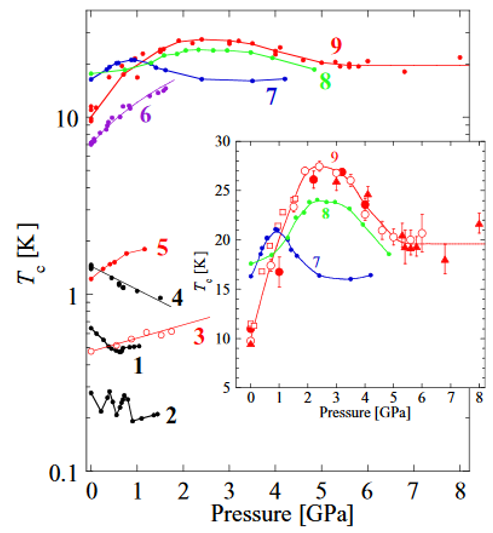
\includegraphics[scale=0.5]{GraphEj.png}
    \caption{El \emph{caption} de esta figura debe tener una descripción detallada de lo que se está mostrando como resultado. Un \emph{caption} que diga ``Gráfica de T vs P'' no dice absolutamente nada de cómo fueron obtenidos los datos y los resultados que se pueden concluir a partir de estos. Siempre los datos deben llevar las respectivas barras de error o indicar que el tamaño de estas es muy pequeño para ser visualizadas. Usar colores como los que se ve en la figura para diferenciar fácilmente los datos. Nunca unir los puntos experimentales, las líneas sólidas están reservadas para los ajustes. No usar notación científica de Excel.}
    \label{fig:my_label}
    \end{figure}

    \item Analizar los resultados expuestos en las tablas y gráficas. Comparar estos resultados con la teoría, objetivos e hipótesis propuestas en la introducción. Se debe reportar si sus resultados y lo que aprendió en la práctica lo lleva a cumplir los objetivos propuestos, si son valores deseables o no; escriba oraciones completas que expresen sus ideas. Si se realizó ajuste, este debe estar referenciado en la gráfica y en el texto (con su respectiva incertidumbre). El cálculo de la incertidumbre del resultado obtenido debe estar situado junto al resultado obtenido, no debe aparecer el resultado al inicio y la incertidumbre al final.
    \item Cuando consultan un valor experimental que se mide con mucha precisión, por ejemplo una constante física, se denomina: \emph{el valor reportado en la literatura} y colocan la referencia (aconsejo la NIST). No usar más \emph{el valor teórico}.
    \item No vuelvan nunca a calcular un error porcentual. Con la incertidumbre y el valor reportado en la literatura pueden hacer un mejor análisis.
    \item Recuerden que todas las incertidumbres llevan 1 cifra significativa (máximo 2 en casos especiales).

\end{itemize}





\section{Conclusiones}

Se deben contestar las preguntas planteadas inicialmente o dar las razones por las cuales no es posible hacerlo. Las conclusiones deben ser necesariamente una consecuencia del experimento realizado, es  decir  que  no  se  deben  tocar  aspectos  que  no  se  hayan  expuesto  en  la  sección  de resultados y análisis. Si escribe algo que no se encuentra en la sección de resultados y análisis,  esto quiere decir que hace falta incluir material en resultados y análisis. Concluir únicamente aspectos pertinentes al trabajo obtenido en el laboratorio; se deben evitar las generalizaciones que no hablan concretamente de lo que lograron o midieron en la práctica experimental. NO USAR ITEMIZE. No reportar resultados nuevos en esta sección, pueden comparar los resultados con los obtenidos por otros autores (por ejemplo sus compañeros o los que encontraron en su revisión bibliográfica).


% IMPORTANTE: Comentar o eliminar la siguiente linea cuando vayan a realizar el INFORME
\bibliographystyle{apalike}


\bibliography{Referencias}
\nocite{Ejemplo}

\section*{Apéndice de cálculo de errores}

Se deben indicar explícitamente los pasos de análisis de error que se hicieron para llegar a al(los) resultado(s). Ejemplo: la propagación de error, incertidumbre en un ajuste de mínimos cuadrados, análisis estadístico, redondeo de cifras significativas, entre otros.

Las fórmulas de cómo se obtuvieron cada uno de los valores reportados debe ser incluido como si el análisis estadístico se hiciera manualmente.
\end{document}
